\documentclass{article}
\usepackage{graphicx}


\begin{document}


% Title Page
\title{Data Collection Documentation (Draft)}
\author{Steven Deutekom}
\date{June 2019}
\maketitle


% Table of Contents
\newpage
\tableofcontents


% Introduction
\newpage
\section{Introduction}
% What are we doing?
The goal of this project is to collect source code samples from individual authors from various online sources. It requires finding samples that have certain sociolinguistic characteristics such as gender, region, and experience. In addition to sociolinguistic characteristics, it is necessary that the samples are the work of only a single author. Data that meets these needs is being collected and used to create a dataset with information on authors and their source code.

% Why are we doing it?
The collected data will be used for sociolinguistic research into how people use programming languages. Current and future University of Lethbridge students will use this research to learn how sociolinguistic characteristics affect how programmers write code. Previous research was conducted with a small dataset of student programs. This new dataset will contain many samples from a larger set of programmers.

% What is coming in this documents?
The document is broken into three main sections. Each section details one of the sources that was used to collect data. First, the collection methods used to gather source code from GitHub. Then, the methods used to collect source code from Codeforces. Lastly, the methods that were used to add gender data to the samples collected.

Each section introduces the sources and collection methods. Then it discusses the pros and cons of the source. Next an overview of the process of collecting data is given, with diagrams to help visualize it. Following this a more in depth technical examination of the collection process takes place. Finally, some reflection on the source is given (needed?).


% Github
\section{Collecting Source Code From GitHub}
% Introduction to the sources being used
% Introduction to the collection strategies
% Pros and Cons of each along with steps taken to try and overcome any issues.
% High level overview of the process w/ diagrams

\begin{figure}[!h]
    \centering
    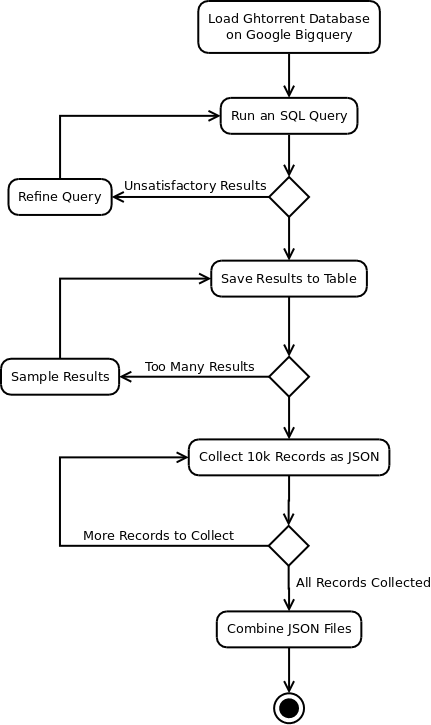
\includegraphics[height=10cm]{diagrams/ght_process.png}
    \caption{Getting Data From Ghtorrent}
\end{figure}

\begin{figure}[!h]
    \centering
    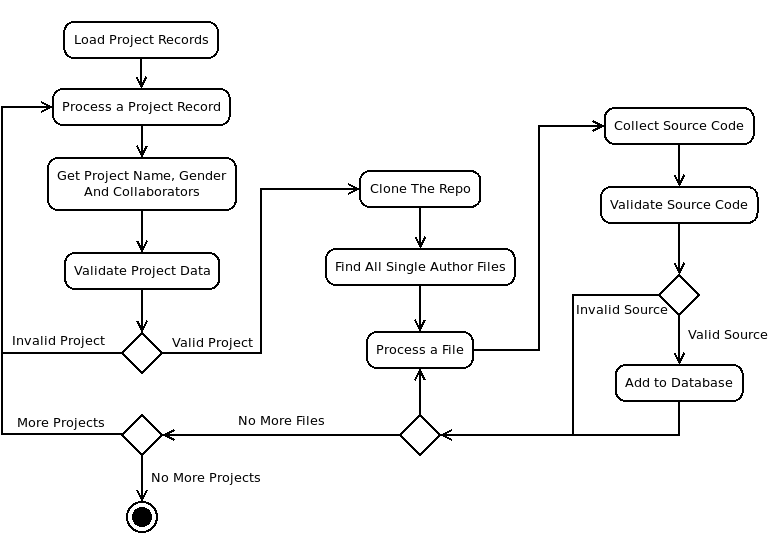
\includegraphics[height=10cm]{diagrams/projects.png}
    \caption{Getting GitHub Project Source Code}
\end{figure}

\begin{figure}[!h]
    \centering
    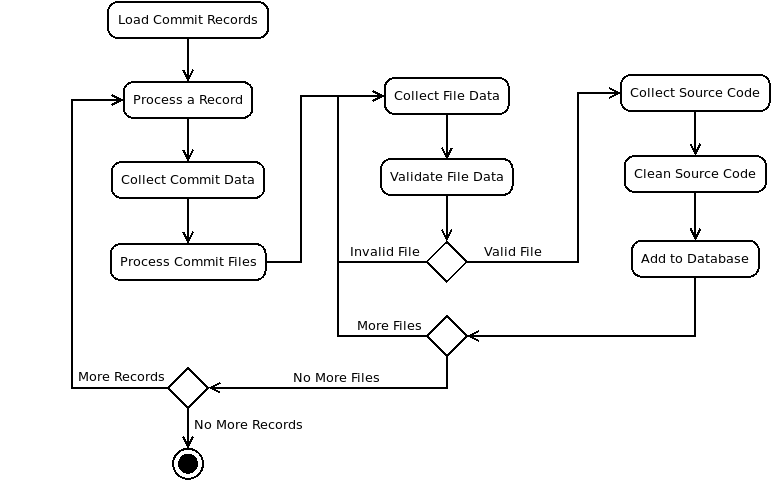
\includegraphics[height=10cm]{diagrams/commits.png}
    \caption{Getting GitHub Commit Source Code}
\end{figure}
% Discussion of each subprocess with technical details and the data it gives and technical issues that are not related to the websites themselves (not listed in pros and cons)


% Codeforces
\section{Collecting Source Code From Codeforces}
% Introduction to the source being used
% Pros and cons of collecting from codeforces along with steps taken to try and overcome any issues.
% High level overview of the process

\begin{figure}[!h]
    \centering
    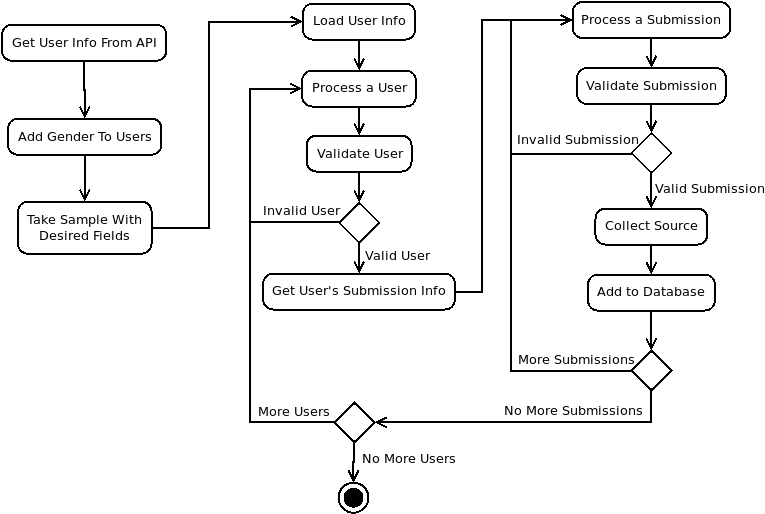
\includegraphics[height=10cm]{diagrams/cf_process.png}
    \caption{Getting Data From Codeforces}
\end{figure}

% Discussion of each subprocess with technical details, the data collected, and the technical issues


% Gender Labeling
\section{Adding Gender Labels to Authors}
% Introduction to the sources being used
% Discussion of the pros and cons and difficulties along with steps taken to try and overcome any issues.
% Overview of the process
% Discussion of the parts of the process (if there are any) and the more technical details, what kind of data was collected, and any technical issues.


% Conclusion
\section{Conclusion}
% Comment on the successes and failures?
% Future improvements or additions


\end{document}